\section{Test}
Vi har delt vores tests op i 2 forskellige tests. Brugertest og programtest.
Vi har lavet en brugertest af 3 forskellige personer. Der er lavet programtest af hhv. terningens tilfældighed, chancekortenes tilfældighed samt antallet af chancekort. Derudover er der også udarbejdet en Coverage dokumentation.
%Lav mindst tre testcases med tilhørende fremgangsmåde/testprocedure og testrapporter.
%Lav mindst én Junit test til centrale metoder. Inkludér code coverage dokumentation.
%Lav mindst én brugertest. Husk at brugeren skal være en der ikke kan kode.

%Brugertesten skal have noget mere struktur. Se link: https://docs.google.com/presentation/d/18r62fV04K8nGgnxyOpVj277v1-kIRZUsXMRZDco-vBk/edit#slide=id.g6b636aa0b1_1_0

%Brugervenlighedstest. evt. fiktiv idk
% https://docs.google.com/presentation/d/1kR6BLZO9P_PZufOLO8ABa-TedmYmsYr75RO45S3bF4M/edit#slide=id.g6ad4536212_0_20
%evt. bare forklar vores brugervenlighed

%Gør det tydeligt hvor mange testpersoner der er, hvilken aldersgruppe og hvor meget kendskab de har til matador og IT generelt
%Bør også noteres rollerne ved observatører 
%Hvor lang tid tog det for dem at gennemføre spillet?
%Blev der begået nogle fejl? Hvilke?


%Er en performancetest mulig?

\subsection{Brugertest}

\subsubsection{Krav til brugertest}
\begin{enumerate}
    \item Observatøren må ikke vejlede før eller under testen.
    \item Testen skal udføres af personer i forskellige aldre.
    \item Der skal være 2-4 testpersoner i samme test.
    \item Testpersonerne skal have en opgave, som observatøren ikke må hjælpe med.
    \item Testbrugerne skal tænke højt under testen.
\end{enumerate}


\subsubsection{Testens udførelse}
Brugertesten er lavet på en far, en mor og deres yngre datter på 12 år. 
Spillet startes nemt og uden problemer. Alle spillere kan skrive sit navn ind i feltet og starte spillet. De første par ture går hurtigt og uden problemer, og alle spillere kan finde ud af spillet. 

Da første spiller landede på et chancekort og fik valget "Ryk frem, eller tag et nyt chancekort" vælger han uden problemer, en af de 2 valgmuligheder og spillet fortsætter.

Testpersonerne fik opgaven: Hvordan finder man ud af hvem der ejer de forskellige ejendomme?
Ved at trykke lidt rundt på pladen, fandt spillerne hurtigt ud af, at man kunne trykke på felterne for at se ejeren af ejendommen. 

\subsubsection{Testrapport}
Undervejs i spillet, blev nogle få fejl opdaget. Dog ikke nogle væsentlige fejl der gjorde det umuligt at spille spillet. 

Eksempelvis, når en spiller skal tage sin tur, kan man se hvis tur det er oppe i venstre hjørne. Når man derefter lander på et chancekort, forsvinder dette. Følger man ikke med i spillet eller hvis tur det er, er det ikke muligt at ikke se, hvis tur det er, før chancekortet er trukket og eventuelle valg er taget. 
En anden småting var, at spilleren ikke kunne vælge farve på deres bil. Første gang de startede spillet, blev både moren og datteren samme farve bil. Det gjorde det svært at spille spillet, da man ikke kunne se hvem der var hvem. Dette kunne fikses ved enten at gøre det muligt for spilleren at vælge farve på bilen, eller ved at gøre det umuligt for 2 spillere at få samme farve bil. 


\clearpage
\subsection{Programtest}
Vi har lavet tre JUnit tests af vores version af matadorspillet. Testene tester hhv. terningens tilfældighed, chancekortene tilfældighed samt test af antallet af chancekortene.

\subsubsection{Test af terningens tilfældighed}
    \begin{figure}[H]
        \centering
        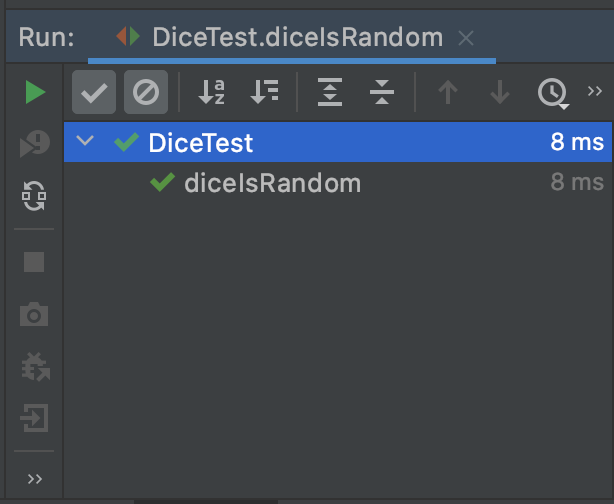
\includegraphics[width=8cm]{figures/diceIsRandomTest.png}
        \caption{JUnit test for at teste tilfældigheden af Dice klassens metode roll()}
        \emph{Testen af Dice klassen og dens roll() metode var en succes. Koden ses i bilag \ref{diceTest}}
    \end{figure}
    Testen af Dice klassen gør brug af et for loop, som køres 100.000 gange. I loopet gør vi brug af Dice klassens roll() metode, for at kaste med terningen. Vi tjekker hver slag, for at se om man slog 1. Efter loopet og de 100.000 slag med terningen, tjekker vi om vi har slået 1 med terningen det forventede antal gange. Vi tester altså om antallet af gange 1 blev slået, afviger væsentligt fra det forvende antal. Gør den det, fejler testen.
    

\subsubsection{Test af chancekort tilfældighed}
    \begin{figure}[H]
        \centering
        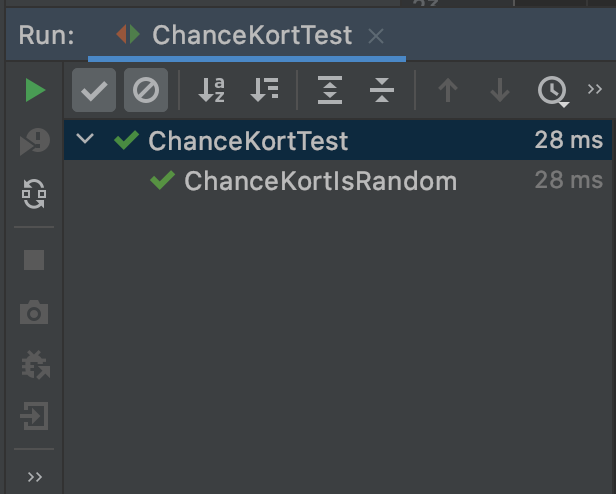
\includegraphics[width=8cm]{figures/chanceKortIsRandom.png}
        \caption{JUnit test for at teste tilfældigheden af ChanceKort klassens metode randomChanceKort()}
        \emph{Testen af ChanceKort klassen og dens randomChanceKort() metode var en succes. Koden ses i bilag \ref{ChanceKortTest}}
    \end{figure}
    Testen her er opbygget på samme måde som testen af Dice klassens tilfældighed. Vi kører randomChanceKort() metoden 100.000 gange og ser om vi fik kort 1 færre eller flere gange end forventet. Denne test er lavet da alle 24 kort var med i spillet, hvilket senere er blevet ændret. For at testen skal have succes, skal der derfor tilføjet alle 24 kort metoder igen. 
    
    
\subsubsection{Test af antal chancekort}
    \begin{figure}[H]
        \centering
        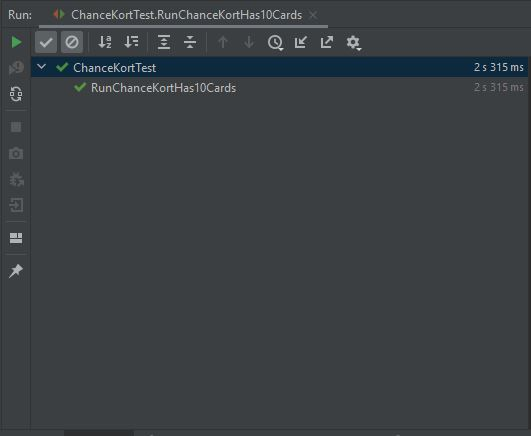
\includegraphics[width=15cm]{figures/RunChanceKortHas10Cards.JPG}
        \caption{JUnit test for at teste at RunChanceKort klassen indeholder det rigtige antal kort.}
        \emph{Testen af RunChanceKort klassen var en succes. Koden ses i bilag \ref{ChanceKortTest}}
    \end{figure}
    Vi har her ændret antal chance kort til 10 i stedet for 24. Her tester vi så antallet af kort, for at sikre at det kun er de 10 kort der er med i spillet. Det gør vi ved at oprette et array med alle de forskellige metoder i RunChanceKort klassen. Vi husker at der er 12 metoder (10 kort() metoder og 2 andre private metoder, som bruges i kort() metoderne). Til sidst sammenligner vi længden af arrayet med det forventede antal ved brug af assertEquals(expected, actual);


\subsubsection{Coverage dokumentation}
\begin{figure}[H]
        \centering
        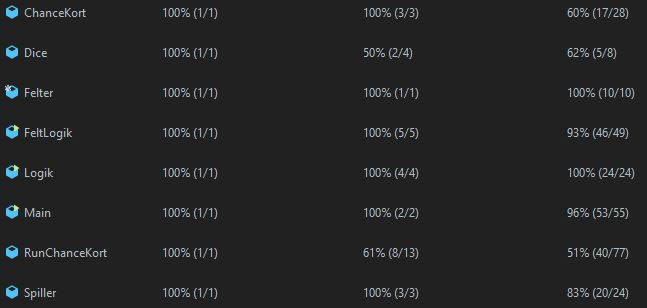
\includegraphics[width=15cm]{figures/codeCoverage.JPG}
        \caption{Code Coverage test}
        \emph{Resultaternes rækkefølge fra venstre til højre er hhv. klasse, metoder og linjer}
    \end{figure}
    Ud over JUnit testene har vi lavet en Code Coverage test, som tester hvor meget af den skrevne kode bliver kørt, når programmet bliver spillet.
    Som resultat af testen bliver alle klasser og 78\% af alle linjer brugt. Dette kan dog variere fra gang til gang, da bl.a. antallet af brugte chancekort ændrer sig. RunChanceKort er derfor den eneste klasse, hvor det vil variere hvor mange af klassens metoder, der vil blive brugt. Da de forskellige chancekort sjældent bliver brugt, har vi valgt, at lave en JUnit test netop til chancekortene så vi ved, at alle chancekort har mulighed for at blive kørt.
    
    \begin{figure}[H]
        \centering
        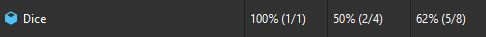
\includegraphics[width=12cm]{figures/diceCoverage.JPG}
        \caption{JUnit Dice Coverage test}
        \emph{Resultaternes rækkefølge fra venstre til højre er hhv. klasse, metoder og linjer}
    \end{figure}
    
    \begin{figure}[H]
        \centering
        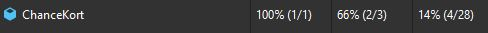
\includegraphics[width=12cm]{figures/chanceCoverage.JPG}
        \caption{JUnit ChanceKort Coverage test}
        \emph{Resultaternes rækkefølge fra venstre til højre er hhv. klasse, metoder og linjer}
    \end{figure}

I de to ovenstående figurer er vist Code Coverage ved hhv. DiceTest og ChanceKortTest. Kun 2/4 af metoderne i Dice og 2/3 af metoderne i ChanceKort bliver kørt ved denne test, da de restende metoder ikke er nødvendige for at køre testen. Testen tager ikke brug af disse metoder, da de ikke er nødvendige for vores program.

